\documentclass[10pt, a4paper, twocolumn]{scrartcl}
\usepackage{cite}  
\usepackage{times}
\usepackage{amsmath}
\usepackage{amsfonts}
\usepackage{amssymb}
\usepackage{graphicx}
\usepackage{listings}
\usepackage{enumitem} % used for list - no spaces between items
\usepackage[english]{babel} % English language/hyphenation
\usepackage[top=2.5cm, bottom=3.2cm, left=2cm, right=2cm, columnsep=0.6cm]{geometry}
\usepackage{color} %red, green, blue, yellow, cyan, magenta, black, white
\definecolor{mygreen}{RGB}{28,172,0} % color values Red, Green, Blue
\definecolor{mylilas}{RGB}{170,55,241}

\usepackage{fancyhdr}
\pagestyle{fancyplain}
\fancyhead{}
\renewcommand{\headrulewidth}{0pt} % Remove header underlines
\fancyfoot[L]{} % Empty left footer
\fancyfoot[C]{} % Empty center footer
\fancyfoot[R]{\thepage} 

\usepackage{tikz}
\usetikzlibrary{shapes.geometric,arrows}

\usepackage{sectsty} % Allows customizing section commands
\sectionfont{\centering\large\textbf}
\subsectionfont{\flushleft\normalsize\normalfont\textbf}
\subsubsectionfont{\flushleft\normalsize\normalfont\textit}
%\allsectionsfont{\centering} % Make all sections centered

\usepackage[toc,page]{appendix}


\setlength\parindent{0pt} % remove all indentations in document

%-------------------------------------------------------------------------------------------------------------------------------------------------------------------------------------%
%	                                                                           BEGIN DOCUMENT
%-------------------------------------------------------------------------------------------------------------------------------------------------------------------------------------%

%-------------------------------------------------------------------------- COVER PAGE -------------------------------------------------------------------------------------%
\begin{document} 

\onecolumn

\newcommand{\horrule}[1]{\rule{\linewidth}{#1}}

	\title{\normalfont \normalsize
		\textsc{University of Witwatersrand, Department of Electrical Engineering} \\ [10pt]
		\horrule{0.5pt} \\ [10pt]
		\huge Test Report \\
		\horrule{2pt} \\ [10pt]}
	\author{\textbf{\normalsize{Luka Cakic (671913), Ronen Freeman (386910), Devin Taylor (603956) and Matthew Marsden (609293)}} \\ [10pt]}
	\date {\normalsize \today}
	
	\maketitle


\section{Introduction}

	Tests were conducted to ensure that the application was functioning as anticipated. One set of tests is to determine whether or not the web application is functioning correctly in terms of HTTP response and request messages, and the second set of tests include determining the specific interaction between objects within the software application.
	
\section{Unit Tests}

	\subsection{Front-End}
	
		Determining whether or not the front-end is fully function revolves primarily around testing the integrity of the HTML files produced. Simple tests were conducted which checked the status codes returned when making HTTP requests as well as interlinking of pages. These tests can be found in the \texttt{Code/test\_suite/front\_end/} folder. \\
		
		The tests were written as HTML interactive tests, therefore simply opening the tests in the browser will determine the status of the tests.
		
	\subsection{Back-End}
	
		The back-end related tests revolved primarily around testing the integrity of the interfacing of the front-end with the database. These included testing the establishment of a connection with the database and interacting with the database. The tests written can be found in the \texttt{Code/test\_suite/back\_end/} folder.\\
		
		In order to execute the tests run the file from command line with the prefix \texttt{php}, i.e. \texttt{php filename.php}.
	
	
\section{HTTP Request and Response Messages}

	Wireshark, a packet sniffer, was used to determine whether or not the Apache server was able to interact with the web browser in loading the application. This was primarily to test the integrity of the HTML web pages designed (their ability to interface with \texttt{css} files and images) as it can be assumed that the Apache server would function correctly. Therefore, any source of error would most likely be as a result of the web pages designed.
	
	\subsection{Localhost Communication}	
	
		A simple test was conducted with loading the \texttt{create\_account.php} file, the HTTP trace sequence can be seen below in Figure~\ref{http_create_account}.
		
		\begin{figure}[h!]
			\centering
			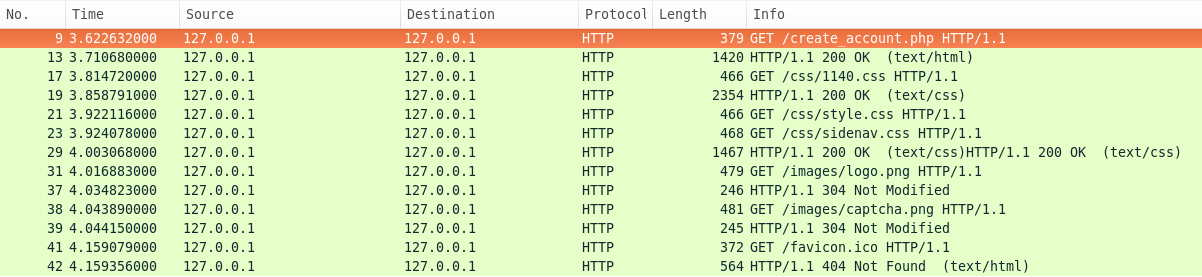
\includegraphics[width = \textwidth]{../images/http_create_account.png}
			\caption{HTTP trace sequence for loading the create account web page}
			\label{http_create_account}
		\end{figure}
		
		From the above image it can be noted that the responses from the server, to all requests, were successful. This indicates that the web pages are correctly formed. Specific mention must be made of trace numbers 19 and 37. These are response messages to GET requests for a \texttt{css} file and an image. Without these two aspects the web page would be malformed.
		
	\subsection{External Software Communication}
	
		It was also necessary to test whether or not the application was correctly interfacing with the external software, Google Maps API, being utilised. The web page \texttt{map\_gen.php} was run which essentially initialised the Google Maps API and processes the requested route. The trace sequence observed can be seen below in Figure~\ref{wireshark_google_maps}.\\
		
		\begin{figure}[h!]
			\centering
			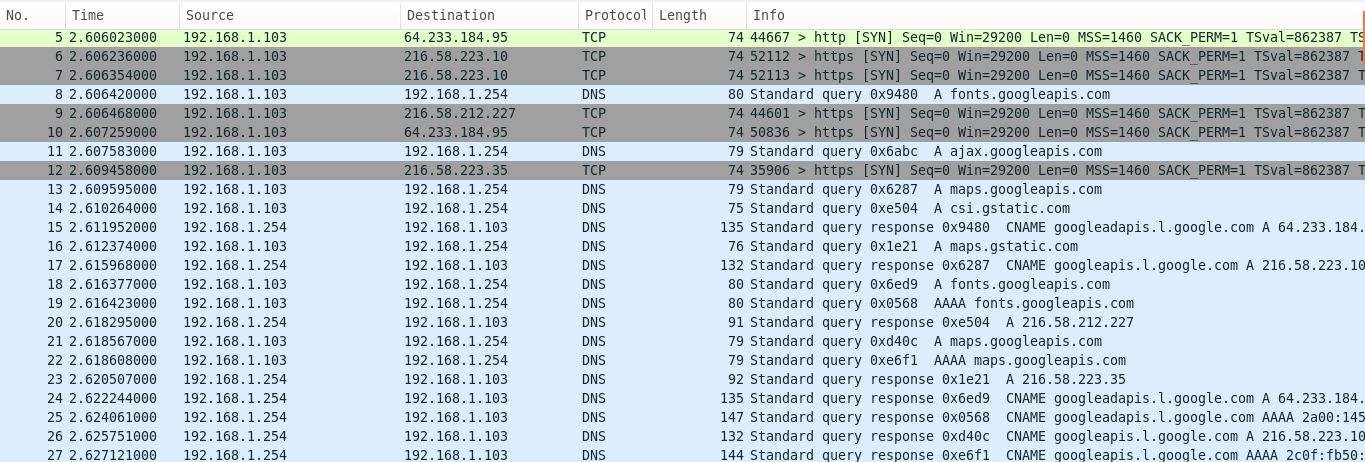
\includegraphics[width = \textwidth]{../images/wireshark_google_maps.png}
			\caption{Trace sequence for Google Maps API requests}
			\label{wireshark_google_maps}
		\end{figure}
		
		Due to the API interaction being HTTPS as opposed to the HTTP observed in Figure~\ref{http_create_account}, the message sequence takes on a different form. Despite this, under the `Info' tab it can be noted that there are `standard query' and corresponding `standard query response' messages. These are the sequences of communication between the Apache server and the Google Maps API server obtaining the necessary information to correctly display the map.

\end{document}